\documentclass[12pt]{article}
\usepackage{sbc-template}
\usepackage[T1]{fontenc}
\usepackage[utf8]{inputenc}
\usepackage{babel}
\babelprovide[import,main]{portuguese}
\addto\captionsportuguese{\renewcommand{\figurename}{Figura}\renewcommand{\tablename}{Tabela}\renewcommand{\refname}{Referências}}
\usepackage{graphicx,url,booktabs,tabularx,array}
\usepackage{hyperref}
\hypersetup{hidelinks}
\providecommand{\tightlist}{\setlength{\itemsep}{0pt}\setlength{\parskip}{0pt}}
\DeclareUnicodeCharacter{00D7}{\ensuremath{\times}}
\DeclareUnicodeCharacter{2212}{\ensuremath{-}}
\sloppy
\title{ProdTime: aplicativo móvel para estimativa de capacidade e prazo na produção de fitas têxteis}
\author{Josué Paulo Alexandrina\inst{1}}
\address{Gran Faculdade\\Análise e Desenvolvimento de Sistemas (ADS)
\email{josue\_jpaej@hotmail.com}}
\begin{document}
\maketitle
\begin{resumo}
Estimativas de capacidade e prazo na produção de fitas têxteis eram calculadas manualmente e, depois, em VBA. Este trabalho apresenta o ProdTime, aplicativo Android em Kotlin e Compose para estimar produção, prazo e viabilidade de metas. O desenvolvimento aplicado envolveu análise do legado, especificação das regras matemáticas e do calendário produtivo e implementação incremental, com validação automatizada e física. Os resultados reproduzem as regressões de 8.846 m e 13.270 m. A contribuição é formalizar regras produtivas rastreáveis em três jornadas móveis. A operação depende das entradas do usuário e não recebe dados de máquinas em tempo real.
\end{resumo}
\textbf{Palavras-chave:} produção têxtil; planejamento da produção; aplicativo móvel; estimativa de capacidade; estimativa de prazo.
\begin{abstract}
Capacity and completion-date estimates in textile tape production relied on manual calculations and later VBA. This paper presents ProdTime, an Android application built with Kotlin and Compose to estimate production, completion dates, and target feasibility. The applied development process involved legacy analysis, specification of mathematical rules and the working calendar, and incremental implementation, with automated and physical-device validation. Results reproduce the regression cases of 8,846 m and 13,270 m. The contribution is the formalization of traceable production rules through three mobile workflows. Operation depends on user inputs and does not receive real-time machine data.
\end{abstract}
\textbf{Keywords:} textile production; production planning; mobile application; capacity estimation; completion-date estimation.

\section{Introdução}\label{introduuxe7uxe3o}

O planejamento da produção têxtil envolve decisões sobre quantidades, recursos e prazos. Uma estimativa de metragem depende de velocidade de produção, quantidade de fitas simultâneas, horas disponíveis, desperdício e dias efetivamente trabalhados. A combinação dessas variáveis exige explicitar as premissas usadas nas respostas à produção e às vendas.

A literatura descreve problemas de planejamento e controle em processos têxteis multifásicos, com múltiplas unidades e requisitos produtivos (KARACAPILIDIS; PAPPIS, 1996), e problemas formais de programação da produção com máquinas ou teares paralelos (SERAFINI; SPERANZA, 1992). Esses trabalhos abordam decisões industriais mais amplas que o recorte deste projeto: estimativas determinísticas de capacidade, prazo e viabilidade para condições produtivas informadas.

No contexto que originou o ProdTime, as estimativas eram realizadas manualmente por profissionais experientes, concentrando conhecimento e podendo atrasar respostas da produção e de vendas. O autor posteriormente desenvolveu uma calculadora integrada a um ERP legado em VBA. Com a substituição desse ERP por um ERP Web, a necessidade específica de cálculo foi isolada no ProdTime, aplicativo móvel cuja integração com o novo ERP permanece futura.

O problema de desenvolvimento consiste em disponibilizar estimativas reproduzíveis em uma interface móvel, preservando as relações matemáticas conhecidas e explicitando calendário e arredondamento. O objetivo é responder quanto pode ser produzido em um período, quando uma quantidade pode ser concluída e se uma meta é atendida, indicando o mínimo e o adicional de fitas necessários sob as mesmas premissas.

O escopo é um MVP Android local, com parâmetros constantes por estimativa e feriados em memória. Sua contribuição consiste em transformar regras antes acopladas ao legado em um domínio testável e rastreável, acessível por três jornadas móveis. O aplicativo não realiza scheduling geral nem substitui ERP ou planejamento e controle da produção (PCP). A avaliação concentra-se na concordância com casos conhecidos e no funcionamento das jornadas; ganhos operacionais não foram mensurados.

\section{Fundamentação e Trabalhos Relacionados}\label{fundamentauxe7uxe3o-e-trabalhos-relacionados}

Karacapilidis e Pappis (1996) abordam planejamento e controle da produção têxtil em processos multifásicos, com múltiplas unidades, horizontes e requisitos produtivos. Esse contexto situa a complexidade das decisões e a necessidade de organizar informações produtivas.

Serafini e Speranza (1992) estudam problemas de scheduling na indústria têxtil, envolvendo máquinas ou teares paralelos, algoritmos, limites e heurísticas. A referência evidencia problemas formais de alocação e programação da produção que ultrapassam o cálculo de capacidade sob parâmetros fixos.

Laoboonlur, Hodgson e Thoney (2006) apresentam um exemplo complementar em tingimento e acabamento de malha, com ambiente flexible job shop, setups dependentes da sequência e family scheduling. Trata-se de outro processo têxtil, cujas características não são equiparadas à produção de fitas.

Hodge et al.~(2011) discutem a adaptação de princípios lean à indústria têxtil, com atenção a desperdícios e atividades sem valor, contextualizando a melhoria sistemática de processos. No ProdTime, desperdício designa o percentual informado para estimar produção líquida; não representa uma perda medida pelo aplicativo.

As referências foram selecionadas para contextualizar planejamento, programação e melhoria de processos no setor. A consulta alcançou metadados e resumos editoriais, sem leitura integral. Elas não validam diretamente o ProdTime: os algoritmos de scheduling citados não foram implementados, e o aplicativo não demonstra adoção integral de lean ou redução mensurada de desperdícios. A avaliação da solução fundamenta-se nos casos de regressão e nas validações descritas a seguir.

\section{Metodologia}\label{metodologia}

O trabalho foi conduzido como desenvolvimento aplicado de software baseado em um problema real e na análise de uma solução legada. A identificação da necessidade e o levantamento do processo manual estabeleceram as perguntas de produção e prazo e a dependência do conhecimento de profissionais experientes. A análise da calculadora VBA permitiu reconstruir as relações entre velocidade, fitas, horas, dias, desperdício e saldo.

A engenharia reversa separou o comportamento histórico da regra desejada para o novo produto. As relações matemáticas foram preservadas com política decimal explícita; coerções implícitas, dependência da interface e subtrações repetidas no calendário foram tratadas como limitações do legado. Em seguida, foram especificados unidades, contratos, duas fronteiras de arredondamento, classificação das datas e resolução de feriados.

A implementação foi conduzida incrementalmente, passando pelo motor matemático, calendário, estimativa de produção, prazo, viabilidade e interface móvel. Testes automatizados verificaram os contratos, regressões históricas e casos de borda; verificações locais avaliaram a execução da suíte JVM e a montagem do aplicativo.

A validação em dispositivo físico verificou as três jornadas, calendário, feriados e interação com os formulários. Achados de cursor, apresentação de viabilidade, cópia e entradas motivaram refinamentos posteriormente verificados. Esse procedimento complementou os testes de cálculo, sem constituir estudo com usuários ou avaliação ampla de compatibilidade.

\section{Desenvolvimento do ProdTime}\label{desenvolvimento-do-prodtime}

\subsection{Arquitetura}\label{arquitetura}

O aplicativo é Android nativo, desenvolvido em Kotlin, com interface em Jetpack Compose e Material 3. O domínio é Kotlin puro, independente de Android e Compose. A interface coleta e valida entradas, coordena o estado e apresenta resultados; as regras produtivas ficam nos componentes de cálculo. A operação é local e não exige backend.

O \texttt{ProductionCapacityCalculator} calcula capacidade, desperdício, produção líquida e saldo. O \texttt{ProductiveCalendarCalculator} classifica as datas do intervalo. O \texttt{HolidayResolver} converte definições de feriados em datas concretas. O \texttt{ProductionEstimateCalculator} integra esses componentes para estimar um período; o \texttt{ProductionDeadlineCalculator} encontra a primeira data suficiente para a meta; e o \texttt{ProductionViabilityAdvisor} compara a estimativa com a meta e determina o mínimo e o adicional de fitas. Essa composição reutiliza as regras comuns nas três jornadas.

A Figura 1 apresenta o acesso às três jornadas do aplicativo.

\begin{figure}[htbp]
\centering
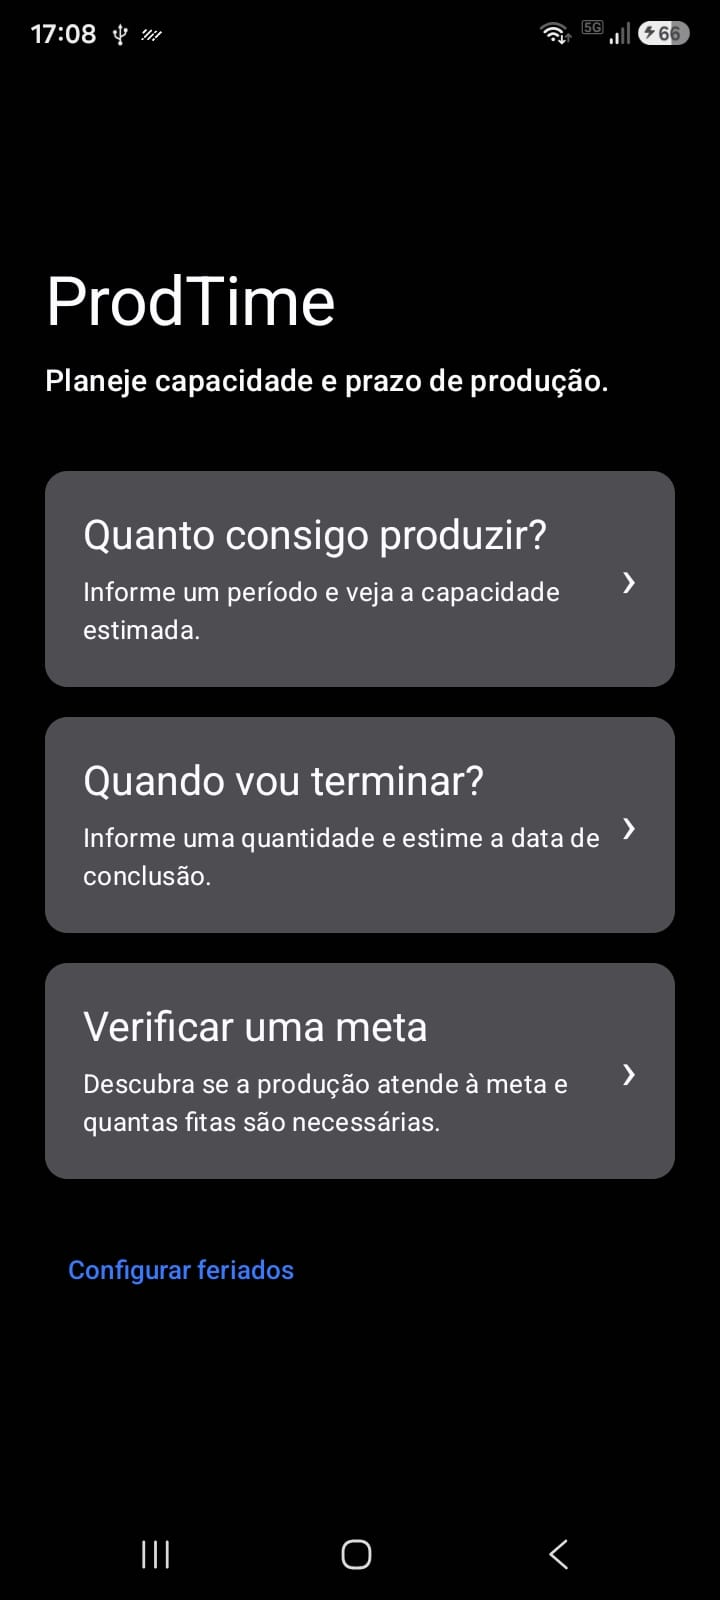
\includegraphics[width=0.40\textwidth,keepaspectratio]{../figures/figura_1_home_prodtime.jpg}
\caption{Tela inicial do ProdTime com acesso às três jornadas.}
\label{fig:1}
\end{figure}

\subsection{Motor de capacidade}\label{motor-de-capacidade}

Considere velocidade \texttt{v} em cm/min, quantidade de fitas simultâneas \texttt{F}, horas produtivas por dia \texttt{H}, dias produtivos \texttt{D} e desperdício percentual \texttt{p}. A conversão é:

\begin{quote}\raggedright
velocidade em m/h = (v × 60) / 100
\end{quote}

O cálculo segue a sequência:

\begin{quote}\raggedright
produção bruta decimal = velocidade convertida × F × H × D

produção bruta = arredondamento integral HALF\_EVEN da produção bruta decimal

desperdício = produção bruta × p / 100

produção líquida decimal = produção bruta − desperdício

produção líquida = arredondamento integral HALF\_EVEN da produção líquida decimal

saldo = produção líquida − meta (quando informada)
\end{quote}

O desperdício incide sobre a produção bruta já arredondada e permanece decimal. O saldo existe somente quando há meta. O total de horas produtivas é \texttt{H\ ×\ D}.

O uso de \texttt{BigDecimal}, construído a partir de texto ou constantes exatas, evita conversões intermediárias por \texttt{Double} ou \texttt{Float}. A política \texttt{HALF\_EVEN} arredonda para o inteiro mais próximo e, em empate, escolhe o inteiro par. Ela é aplicada somente às fronteiras bruta e líquida descritas, preservando os resultados históricos conhecidos sem truncamento arbitrário. Horas fracionárias são aceitas, e o domínio não incorpora valores padrão da interface.

\begin{table}[htbp]
\centering
\caption{Principais parâmetros das jornadas.}
\begin{tabularx}{\textwidth}{@{}>{\raggedright\arraybackslash}p{0.23\textwidth} >{\raggedright\arraybackslash}p{0.28\textwidth} >{\raggedright\arraybackslash}X@{}}
\toprule
Parâmetro & Unidade & Papel \\
\midrule
Velocidade & cm/min & Velocidade linear convertida para o cálculo de capacidade. \\
Fitas & unidade & Quantidade de fitas produzidas simultaneamente. \\
Horas produtivas & h/dia & Jornada produtiva aplicada aos dias considerados produtivos. \\
Desperdício & \% & Parcela da produção bruta descontada na estimativa líquida. \\
Período & data & Delimita o calendário na estimativa e na viabilidade; o prazo recebe a data inicial. \\
Meta & m & Quantidade desejada nos fluxos de prazo e viabilidade. \\
\bottomrule
\end{tabularx}
\end{table}

\subsection{Calendário e feriados}\label{calenduxe1rio-e-feriados}

O calendário usa \texttt{LocalDate}, com intervalo-base inclusivo e início não posterior ao fim. As opções de inclusão das pontas são aplicadas antes da classificação produtiva. Em um intervalo de uma única data, ambas as pontas precisam estar incluídas. Cada data restante é avaliada uma vez conforme as políticas de sábados, domingos e feriados.

Trabalhar em feriados remove apenas o impedimento associado ao feriado; não torna produtivo um sábado ou domingo que continue excluído. Colisões entre fim de semana e feriado não geram dupla subtração. As contagens informativas podem se sobrepor, mas a decisão produtiva é única por data. Um calendário válido pode retornar zero dias produtivos; a integração de estimativa trata esse caso com produção zero.

Os feriados cadastrados têm nome e são anuais, por dia e mês, ou de data específica. O \texttt{HolidayResolver} resolve as ocorrências do intervalo e entrega um conjunto de datas ao calendário, deduplicando definições coincidentes. Um feriado anual em 29/02 ocorre somente nos anos bissextos, sem deslocamento para outra data nos anos comuns. Não há carregamento automático de feriados externos. A coleção é compartilhada pelas jornadas durante a sessão e descartada quando o processo termina.

\subsection{Estimativa de produção}\label{estimativa-de-produuxe7uxe3o}

A jornada ``Quanto consigo produzir?'' recebe período, velocidade, fitas, horas produtivas por dia, desperdício e políticas de calendário. O sistema resolve os feriados, identifica os dias produtivos e calcula a capacidade do período. A saída principal é a produção líquida estimada, acompanhada de produção bruta, desperdício e detalhes do calendário. Esse fluxo não utiliza uma meta nem procura uma data de conclusão.

A Figura 2 corresponde ao cenário de três fitas apresentado na validação das regressões.

\begin{figure}[htbp]
\centering
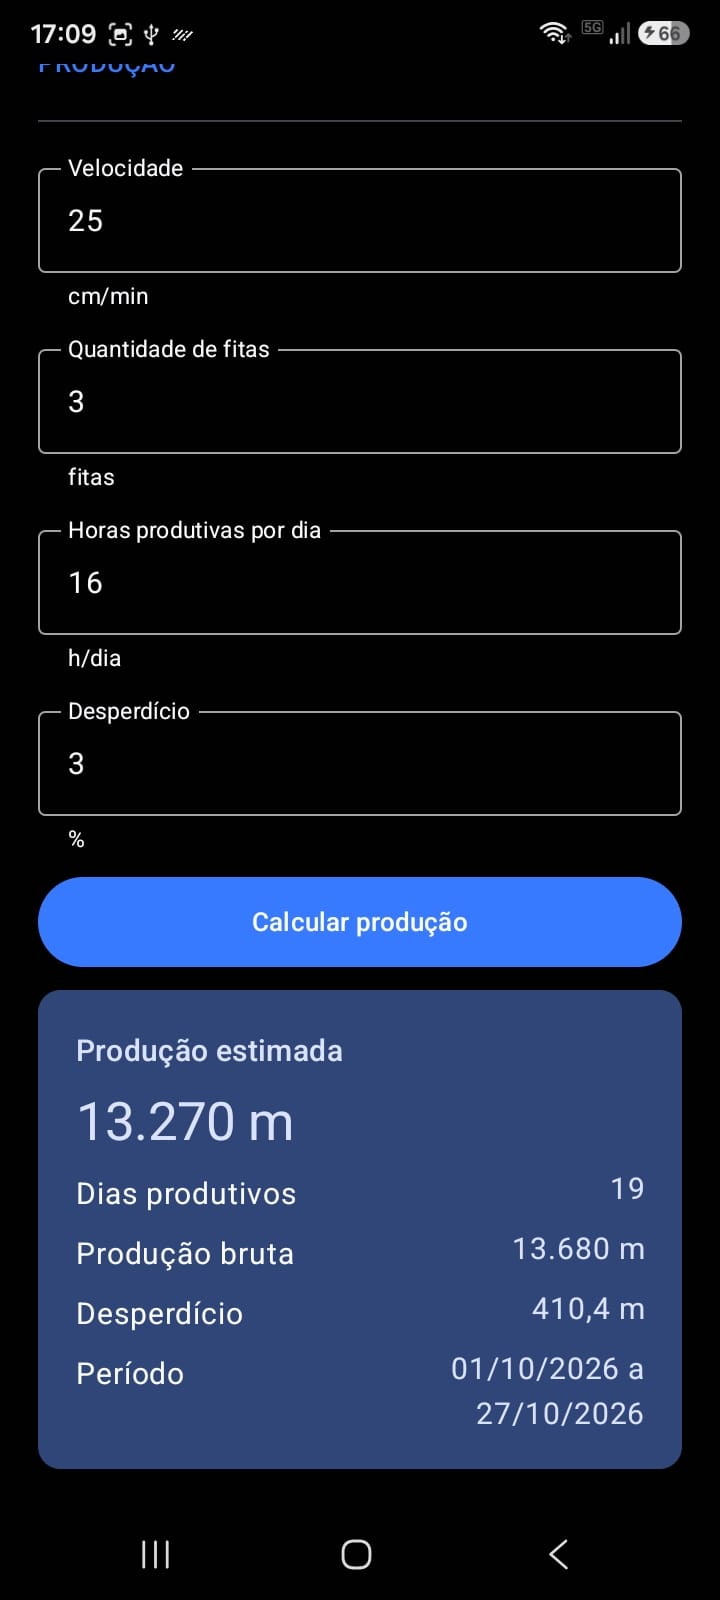
\includegraphics[width=0.40\textwidth,keepaspectratio]{../figures/figura_2_estimativa_13270m.jpg}
\caption{Estimativa de 13.270 m líquidos em 19 dias produtivos, de 01/10/2026 a 27/10/2026.}
\label{fig:2}
\end{figure}

\subsection{Estimativa de prazo}\label{estimativa-de-prazo}

A jornada ``Quando vou terminar?'' tem como entradas meta positiva em metros inteiros, data inicial, condições produtivas e políticas de calendário; a data final não é informada pelo usuário. O \texttt{ProductionDeadlineCalculator} percorre progressivamente as datas e, a cada novo dia produtivo, aplica o mesmo motor de capacidade ao total acumulado de dias. A busca termina na primeira data cuja produção líquida atinge ou supera a meta, respeitando calendário e feriados. A data de conclusão é um resultado e delimita o calendário apresentado. Um horizonte técnico finito impede busca indefinida; a resposta inclui dias produtivos, produção na conclusão e saldo.

A Figura 3 corresponde ao cenário de conclusão da meta de 10.000 m descrito na validação do prazo.

\begin{figure}[htbp]
\centering
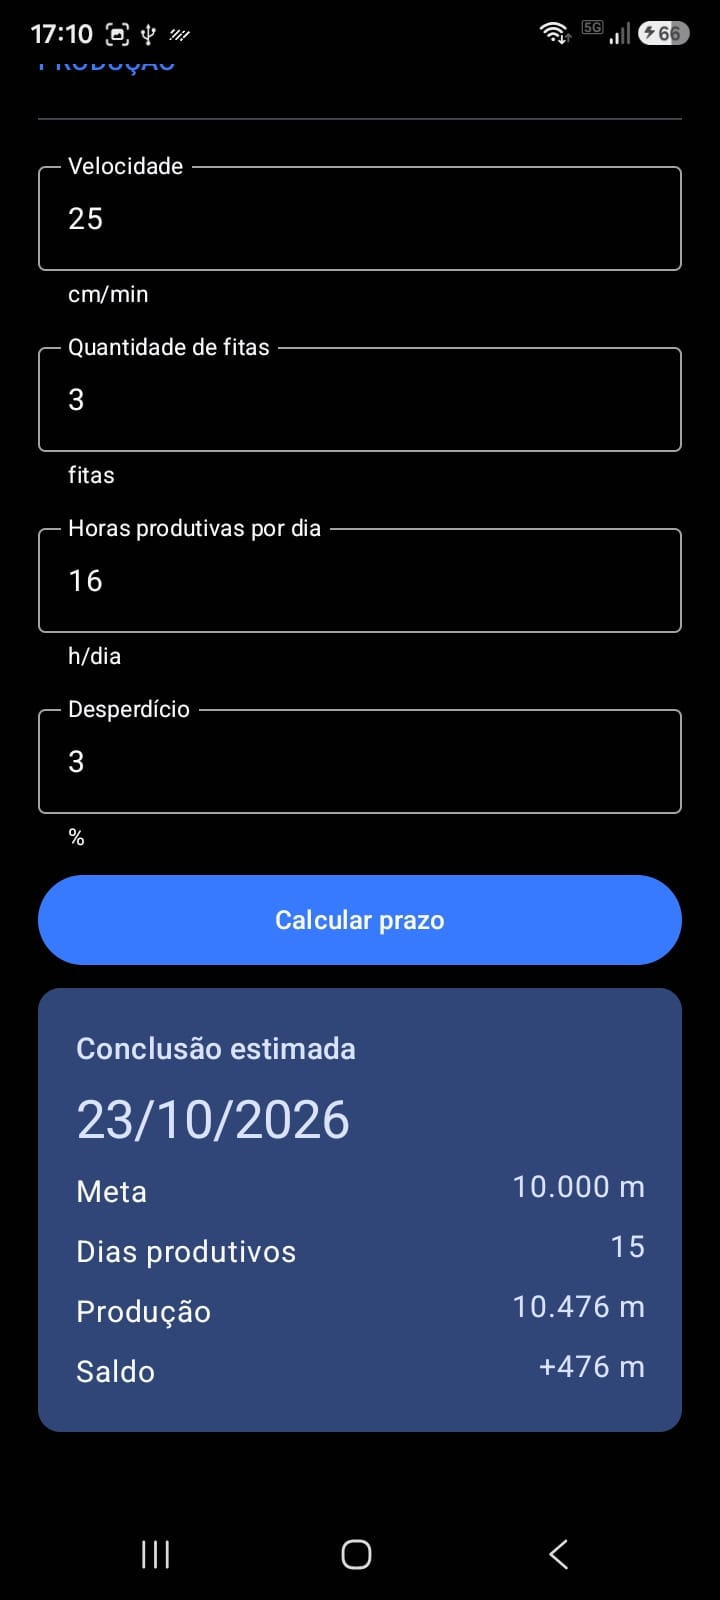
\includegraphics[width=0.40\textwidth,keepaspectratio]{../figures/figura_3_prazo_23102026.jpg}
\caption{Conclusão estimada em 23/10/2026, com 10.476 m em 15 dias produtivos e saldo de +476 m.}
\label{fig:3}
\end{figure}

\subsection{Viabilidade da meta}\label{viabilidade-da-meta}

A jornada de verificação de meta compara a produção líquida estimada no período com a quantidade desejada. O resultado informa atendimento, excedente ou déficit, quantidade mínima de fitas suficiente e quantidade adicional em relação à configuração atual. O mínimo é encontrado reutilizando o motor de capacidade e sua política de arredondamento, mantendo fixos os demais parâmetros. Em um período sem dias produtivos, a recomendação de fitas não é aplicável.

A análise é determinística e condicionada às entradas. Não considera disponibilidade real de máquinas nem executa otimização de PCP; não utiliza IA. A indicação de fitas adicionais expressa uma condição calculada, cuja disponibilidade precisa ser avaliada pelo usuário.

A Figura 4 corresponde à análise da meta de 10.000 m com duas fitas.

\begin{figure}[htbp]
\centering
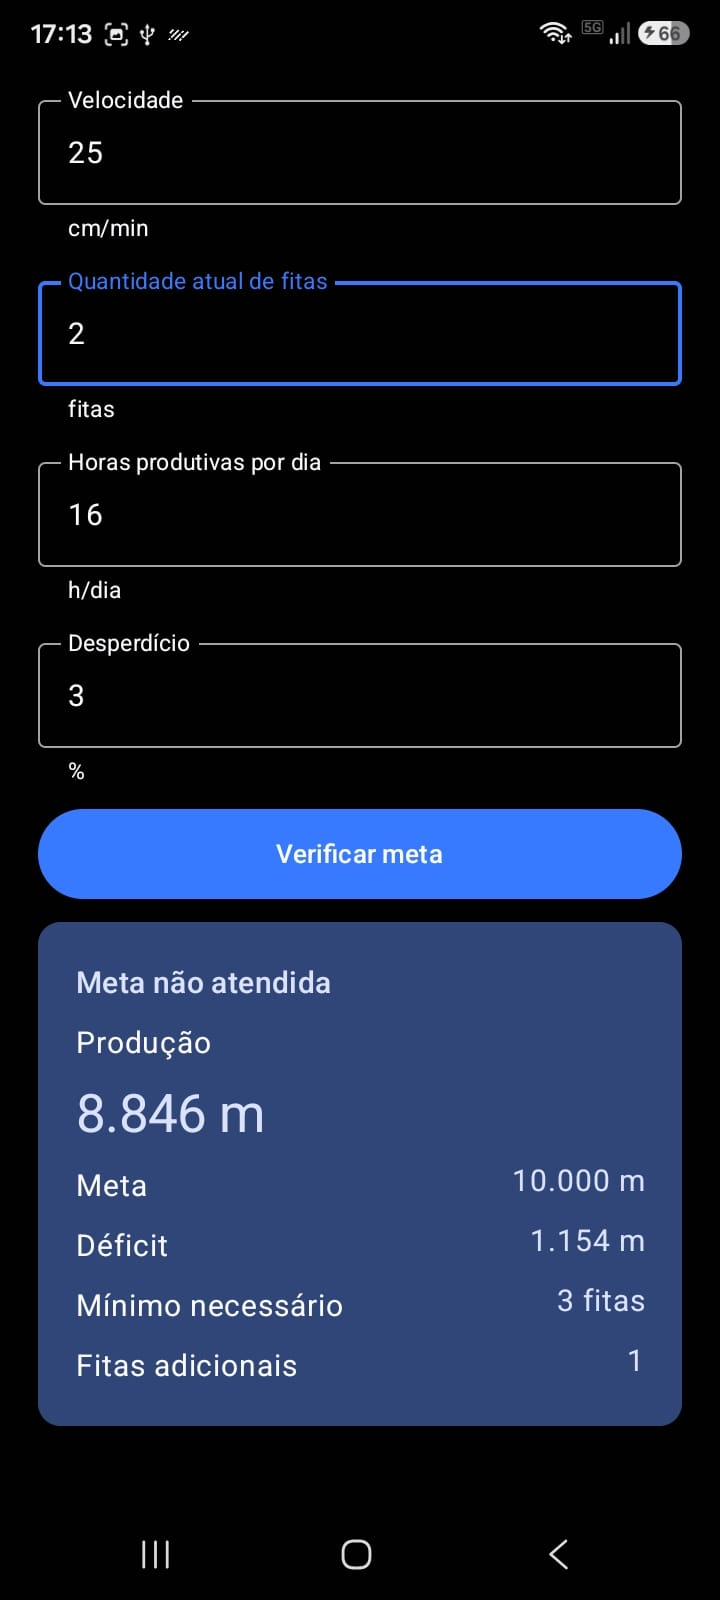
\includegraphics[width=0.40\textwidth,keepaspectratio]{../figures/figura_4_viabilidade_deficit_1154m.jpg}
\caption{Déficit de 1.154 m com duas fitas: mínimo necessário de três fitas e uma fita adicional.}
\label{fig:4}
\end{figure}

\subsection{Interface móvel e robustez das entradas}\label{interface-muxf3vel-e-robustez-das-entradas}

A tela inicial oferece acesso às três jornadas e à configuração de feriados. Os formulários Compose organizam unidades, opções e mensagens de erro; ações de teclado conduzem o foco e o cursor. A apresentação utiliza temas claro e escuro, semântica de acessibilidade, layouts roláveis e feedback textual para resultados e viabilidade. Os resultados podem ser copiados.

A entrada numérica aceita separador decimal por vírgula ou ponto. A sanitização remove espaços em branco e caracteres invisíveis previstos antes da conversão numérica, preservando a rejeição de texto inválido. Limites operacionais de velocidade, fitas, horas, desperdício e meta são verificados na apresentação, sem modificar as fórmulas do domínio. A edição limpa o erro do campo corrigido, permitindo retomar o cálculo sem sair da tela.

\section{Resultados e Validação}\label{resultados-e-validauxe7uxe3o}

Foram comparados resultados calculados com referências históricas e verificados cenários de prazo, viabilidade e feriados. A Tabela 2 sintetiza os casos; as subseções explicam suas condições e interpretação. A concordância observada nesses exemplos não estabelece uma taxa de acerto para produção real.

\subsection{Regressões históricas}\label{regressuxf5es-histuxf3ricas}

As regressões utilizam 25 cm/min, 16 h/dia, 19 dias produtivos e 3\% de desperdício, com duas e três fitas. Os resultados brutos, o desperdício e a produção líquida constam da Tabela 2. Antes do arredondamento líquido, os valores são 8.846,4 m e 13.269,6 m, respectivamente. A política integral produz 8.846 m e 13.270 m, reproduzindo os resultados conhecidos da calculadora VBA. Os testes de regressão verificam esses exemplos sob as condições indicadas.

\subsection{Validação do prazo}\label{validauxe7uxe3o-do-prazo}

Para a meta de 10.000 m, início em 05/10/2026, velocidade de 25 cm/min, três fitas, 16 h/dia e desperdício de 3\%, foi utilizado calendário sem sábados, domingos ou feriados. A conclusão calculada foi 23/10/2026, após 15 dias produtivos, com produção de 10.476 m e saldo de +476 m. O teste de minimalidade verifica que 14 dias são insuficientes e 15 são suficientes nesse cenário.

\subsection{Validação da viabilidade}\label{validauxe7uxe3o-da-viabilidade}

A verificação de meta utiliza 01/10/2026 a 27/10/2026, com 19 dias produtivos, meta de 10.000 m e as demais condições das regressões. Três fitas atendem à meta, enquanto duas são insuficientes. Em ambos os casos, o mínimo calculado é três, com adicionais zero e um, respectivamente. A Tabela 2 reúne os valores de excedente e déficit; a indicação não pressupõe disponibilidade operacional das fitas adicionais.

\subsection{Validação do calendário e dos feriados}\label{validauxe7uxe3o-do-calenduxe1rio-e-dos-feriados}

No cenário de 01/12/2026 a 31/12/2026, com 28 cm/min, uma fita, 16 h/dia e 3\% de desperdício, a política de trabalho em feriado alterou a contagem produtiva de 22 para 23 dias. A produção líquida passou de 5.737 m para 5.997 m, conforme a validação física. O efeito observado limita-se às condições desse cenário.

\begin{table}[htbp]
\centering
\caption{Síntese dos casos documentados de validação.}
\begin{tabularx}{\textwidth}{@{}>{\raggedright\arraybackslash}p{0.23\textwidth} >{\raggedright\arraybackslash}p{0.28\textwidth} >{\raggedright\arraybackslash}X@{}}
\toprule
Caso & Entrada principal & Resultado \\
\midrule
Regressão 2 fitas & 25 cm/min; 16 h/dia; 19 dias; 3\% & 9.120 m brutos; 273,6 m de desperdício; 8.846 m líquidos. \\
Regressão 3 fitas & Mesmas condições; 3 fitas & 13.680 m brutos; 410,4 m de desperdício; 13.270 m líquidos. \\
Prazo & Meta 10.000 m; início 05/10/2026; 3 fitas; 25 cm/min; 16 h/dia; 3\% & 23/10/2026; 15 dias produtivos; 10.476 m; saldo +476 m. \\
Viabilidade 2 fitas & Meta 10.000 m; condições da regressão & Não atende; déficit 1.154 m; mínimo 3; adicional 1. \\
Viabilidade 3 fitas & Meta 10.000 m; condições da regressão & Atende; excedente +3.270 m; mínimo 3; adicional 0. \\
Feriado não trabalhado & Dezembro/2026; 28 cm/min; 1 fita; 16 h/dia; 3\% & 22 dias produtivos; 5.737 m líquidos. \\
Feriado trabalhado & Mesmas condições; política de trabalho alterada & 23 dias produtivos; 5.997 m líquidos. \\
\bottomrule
\end{tabularx}
\end{table}

\subsection{Testes e validação física}\label{testes-e-validauxe7uxe3o-fuxedsica}

Na versão avaliada, a suíte JVM continha 118 métodos anotados com \texttt{@Test}. Essa contagem descreve as fontes, não o total executado em uma tarefa. Os testes abrangem capacidade e \texttt{HALF\_EVEN}, calendário e pontas, recorrência e deduplicação de feriados, estimativa, prazo, viabilidade, conversão numérica, sanitização, limites e apresentação.

Na validação local final, \texttt{testDebugUnitTest} e \texttt{assembleDebug} foram concluídas com \texttt{BUILD\ SUCCESSFUL}. Os registros incluem tarefas reportadas como atualizadas, de modo que a conclusão bem-sucedida não implica reexecução de todos os métodos. Também não permite determinar cobertura percentual.

A validação física foi realizada em um Samsung SM-A066M, verificando as três jornadas, calendário, feriados e interação. Foram registrados e posteriormente aprovados refinamentos de cursor, cópia, limites, sanitização e feedback. Trata-se de funcionamento nos cenários verificados em um aparelho real, sem avaliação ampla de compatibilidade ou estudo com usuários.

\section{Limitações e Trabalhos Futuros}\label{limitauxe7uxf5es-e-trabalhos-futuros}

\subsection{Limitações atuais}\label{limitauxe7uxf5es-atuais}

O aplicativo opera localmente, sem backend, e os feriados cadastrados não persistem após o encerramento do processo. Velocidade, horas, fitas, desperdício e calendário dependem das informações fornecidas pelo usuário. O sistema não recebe dados de máquinas em tempo real e assume condições constantes na estimativa, sem modelar ocupações, liberações ou capacidade variável por intervalo.

Os resultados representam estimativas condicionais, não promessas operacionais. O MVP não utiliza inteligência artificial nem oferece PCP. A validação disponível reúne regressões, testes e observações físicas documentadas; não inclui avaliação quantitativa de economia de tempo, redução de desperdício, desempenho industrial ou estudo abrangente de usabilidade.

\subsection{Trabalhos futuros}\label{trabalhos-futuros}

As possibilidades de evolução incluem integração com ERP Web e PCP, consulta à disponibilidade de máquinas, modelagem de capacidade variável, persistência de feriados e histórico de estimativas. IA para análise de históricos e IoT para obtenção de dados produtivos são possibilidades posteriores, não funcionalidades atuais. Cada evolução exige requisitos, dados e validação próprios; não decorre automaticamente da implementação determinística do MVP.

\section{Conclusão}\label{conclusuxe3o}

O ProdTime implementa estimativa de produção em um período, estimativa da primeira data de atendimento de uma quantidade e avaliação determinística de viabilidade, com indicação do mínimo e do adicional de fitas. A separação entre interface móvel e domínio permite aplicar as mesmas regras de capacidade, calendário e feriados às três jornadas. Os casos documentados reproduzem os resultados históricos de duas e três fitas e apresentam respostas coerentes para prazo, viabilidade e política de feriados.

Os registros de testes e montagem do aplicativo, complementados pela validação em dispositivo físico, sustentam o funcionamento nos cenários analisados. A contribuição se limita à explicitação das regras e à implementação móvel rastreável. A operação local, a ausência de persistência de feriados e de dados em tempo real e a dependência das entradas restringem seu uso a estimativas sob premissas informadas. Não se demonstra ganho operacional quantitativo; integrações e recursos de planejamento ampliado permanecem trabalhos futuros.
\makeatletter
\renewcommand{\@biblabel}[1]{}
\makeatother
\begin{thebibliography}{4}
\bibitem[]{ref1}
HODGE, George L.; GOFORTH ROSS, Kelly; JOINES, Jeff A.; THONEY, Kristin. Adapting lean manufacturing principles to the textile industry. \emph{Production Planning \& Control}, v. 22, n.~3, p.~237--247, 2011. DOI: \href{https://doi.org/10.1080/09537287.2010.498577}{10.1080/09537287.2010.498577}.

\bibitem[]{ref2}
KARACAPILIDIS, Nikos I.; PAPPIS, Costas P. Production planning and control in textile industry: a case study. \emph{Computers in Industry}, v. 30, n.~2, p.~127--144, 1996. DOI: \href{https://doi.org/10.1016/0166-3615(96)00038-3}{10.1016/0166-3615(96)00038-3}.

\bibitem[]{ref3}
LAOBOONLUR, P.; HODGSON, T. J.; THONEY, K. A. Production scheduling in a knitted fabric dyeing and finishing process. \emph{The Journal of The Textile Institute}, v. 97, n.~5, p.~391--399, 2006. DOI: \href{https://doi.org/10.1533/joti.2006.0145}{10.1533/joti.2006.0145}.

\bibitem[]{ref4}
SERAFINI, Paolo; SPERANZA, M. Grazia. Production scheduling problems in a textile industry. \emph{European Journal of Operational Research}, v. 58, n.~2, p.~173--190, 1992. DOI: \href{https://doi.org/10.1016/0377-2217(92)90205-N}{10.1016/0377-2217(92)90205-N}.
\end{thebibliography}
\end{document}
